\chapter{Background Estimation Methods}
Production processes with final states that look similar to the signal process are known as backgrounds. Selections are set with the intent of reducing backgrounds as much as possible (purity), while not eliminating the signal (efficiency). These selections were described in Sec~\ref{ch:EventSelections}. The backgrounds manage to pass the selections due to a variety of reasons, some of which are outlined in Sec~\ref{sec:background_sources}. During the course of measuring a production processes's cross section (in this case \ttZ), the number of signal events passing the selections is important in determining the cross section. Total measured events passing the cross section will contain both signal events as well as background events. Methods, must be developed to estimate the total number of background events so that that total may be subtracted in order to achieve an estimate of the total number of signal events. The following chapter discusses a variety of methods used to estimate the backgrounds to the measurement of the \ttZ cross section in a 3 lepton final state.\\


	\section{Monte Carlo Based Estimation}
	\label{sec:irreducible_estimation}
	
	Monte Carlo simulations rely on a probabilistic theory to to produce single outcomes repeatedly. With enough repetitions of the simulation, the full distribution of outcomes may be shown. This method of simulation maps perfectly onto particle physics as the probabilistic underpinning matches that of Quantum Mechanics and Quantum Field Theory and the repeated simulations matches the repeated collisions. Thus one simulated outcome is an ``event" the same way that one collision in the detector is an event. Monte Carlo simulations of physics process usually are produced in much more abundance that the processes being measured in data, as those processes tend to be statistically limited and not show a smooth distribution. The MC events are then down weighted so that they may when integrated predict the same number of events as measured in data while showing a smoother distribution.\\
	
	MC simulations rely on physical theory and the current state of QFT to calculate matrix elements. From these matrix elements the probabilistic outcomes are determined, and outcomes are chosen. However, it would be beyond current technology to produce a matrix element that covers all collisions and outcomes, so only interesting ones are made and produced (for example a \ttZ sample or \WZZ sample). Further simplifications are made to the computation manageable. Higher order diagrams may be dropped as they cause the computation time to explode but generally contribute only very small amounts to the probability and other simplifications are made. For the majority of the samples used here, this is done with the Madgraph5 MC simulator.\\
	
	The simulated events are then put through a second MC system that evolves the particles over time and cause them to further decay, hadronize, and interact. More assumptions and simplifications are made here as this is a very computationally intensive process. The Pythia6 MC simulator is used for this step on the samples used here. Finally  all of this output is fed into another MC system that simulates particle interaction with matter so as to simulate what happens as these particles travel through the detector. Again more simplifications are made. The simulation of the interaction with the detector depends very heavily on the accuracy and granularity of the detector model used and the bill of materials listed. ATLAS for example has a much more detailed model of the ATLAS detector and thus is thought to generally have slightly more accurate results. This comes at the cost computational time. CMS, however, has slightly less accurate simulations but is able to produce them much faster which helps with producing new samples or reproducing old ones that may need something fixed in them.\\
	
	In all cases, to help cover some of the shortcomings in the simulation methods, some free parameters are tinkered with that cause the simulation to match up with control regions in data. These MC simulations actually end up being amazingly predictive for the shape and frequency of data events. However, they are most accurate with well measured and well understood processes, which is unfortunate as the goal is to measure not well understood or new processes. Thus MC simulations must be relied on in carefully chosen situations. These simulations are very good at showing top production or boson production and their decay chains into quarks and leptons. Thus, in the absence of a method to estimate from data the contribution of the irreducible background sources, these irreducible background sources will be estimated using MC simulation. The irreducible sources are largely multi-boson samples and tops with bosons. A large error is assessed on the cross sections used to normalize these samples as the cross sections have not been measured yet for the processes they simulate as well as extra systematic errors associated with the specific MC generators used. See Secs~\ref{sec:irreducible_sources} and~\ref{ch:eff_and_unc} for more details on how the errors are assessed.
	
	\subsection{Irreducible Sources}
	\label{sec:irreducible_sources}
        		The irreducible sources are difficult to estimate with a data derived method as they appear the same as the signal. They all have the same number of leptons, similar momentum distributions, similar number of jets and jets from b-quarks, and similar \met. Thus a purely theoretical method is relied on.\\ 
		
        
Monte Carlo simulations are used to estimate contributions from the following SM production processes with genuine isolated tri-leptons:

\begin{itemize}
\item \WZZ, \ttWW, \ttW, \tbZ, \ttG, and \ttH with three real leptons in the final state.
\item \ZZZ with four real leptons (one of which is out of acceptance or fails identification or isolation) and two b-tags.
%\item $W\gamma$ with one real lepton and a photon conversion. 
%This background is a priori not estimated by the fake rate method
%because the photon is generally isolated. 
%In practice, this background is completely negligible.
\end{itemize}




Details on the samples used and the corresponding cross sections can be found in Table~\ref{tab:IrreducibleMCSamples}.  
We assign a 50\% uncertainty to the expected number of events from these samples.\\
		
		\subsubsection{Yields of Irreducible Events Predicted in Monte Carlo}
		
Scale factors are applied to MC predictions to account for differences in lepton selection efficiency and $b$-tagging efficiency between data and simulation. See Table ~\ref{tab:irreducible_yields} for a list of background estimates taken from pure MC.\\
%For the MC predictions, the trigger efficiency (Section 5), the MC scale factor for leptons (Section 6.6.1) and the MC scale factor for b-jets (Section 6.6.2) are applied.
%A re-weighting procedure will be applied to account for the difference between PU from these MC samples and the final dataset.



\begin{table}[ht!]
\caption{\label{tab:irreducible_yields} Pure MC normalized to  \intLumi \ and scaled by differences between lepton selection efficiencies in Data and MC as well as b-tag efficiencies.}

\begin{center}
\begin{tabular}{c|c}\hline
&Yields \\
\hline \hline
 \WZZ                                   &  0.05$\pm$0.01 \\
 \ZZZ                                    &  0.01$\pm$0.00 \\
 \ttG                                      &  0.02$\pm$0.02 \\
 \ttWW                                 &  0.02$\pm$0.00 \\
 \ttW                                     &  0.21$\pm$0.07 \\
 \tbZ                                     &  0.42$\pm$0.02 \\
 \ttH                                      &  0.27$\pm$0.02 \\
\hline
Total &  0.98$\pm$0.08 \\
\hline
\end{tabular}
\end{center}
\end{table}
		
		
		
		
		
		
		
		
		
		
		
		
	\section{Data Derived Estimation}
	\label{sec:datadriven}
	Two data driven methods are used to estimate backgrounds which arise due to 1) fake leptons causing an event to pass the selections (e.g. \ttbar \ plus 1 Fake Lepton from a jet) and 2) b-tags that do not come from a vector boson or top decay (e.g. WZ with b-tags possibly from a gluon). As described in Sec~\ref{sec:irreducible_estimation}, processes like these that are on the fringe and rely on less well understood production methods are not as well estimated in MC simulations. Thus, methods were developed to estimate them from data control regions.\\
	\subsection{Estimation of Events Passing Selections Due to Fake Leptons}
	\label{sec:fake_estimation}
        		\subsubsection{Sources of Fake Leptons}
		Typically, fake muons come from decaying heavy flavor partons such as b-quarks. This may occur as a bound state containing a b-quark decays to a bound state containing a c-quark via a virtual W. This W may then decay to an electron or a muon about 22\% of the time. This is actually a lepton then, and will pass most of the lepton selections. The most likely ways to reject it are based on it's displacement from the primary vertex and based on the energy in the cone around it (isolation). However, some times the decay occurred early and the lepton was produced close to the primary vertex and if it also contained most of the energy from the decay, then it will be isolated. In this case it will pass the lepton selections.\\
		
		Fake electrons also arise in the manner described above, but may also come from light flavor decay. If a light flavor jet produces a $\pi^0$ and a charged pion ($\pi^{\pm}$) at the same time, then the charged pion will leave a track, and the $\pi^0$ will decay to photons which will shower electromagnetically. If the track from the charged pion is matched to the shower from the $\pi^0$, this may appear to be an electron when it is not.\\
		
		Fake leptons depend heavily on the momentum of the progenitor particle and on the momentum fraction received by the fake lepton. If the lepton receives a majority of the momentum, then it will be largely on it's own when it leaves energy in the detector and appear to be isolated. This also occurs if the lepton is produced at a large angle of separation to the trajectory of the bulk of the progenitors decay products.\\
		
		An independent sample could be used to measure the rate at which a fake lepton that passes a looser, fake dominated selection will also pass the full measurement lepton selection. This rate is assumed to be universal and applicable to a wide variety of underlying processes, and thus the rate of fake leptons passing selections in a control region should be the same as those in the signal region.\\
		
       		\subsubsection{Overview of Fake Rate Method and Selections}
		In this method, we measure two types of leptons: a ``numerator" lepton passing the full analysis lepton identification and isolation requirement  and a "denominator" lepton passing the analysis selections with relaxed isolation and impact parameter requirement. The ratio of numerator objects to denominator objects is known as a ``fake rate," ``FR," or ``tight to loose ratio."  The fake rate is measured in an independent data sample of multi-jet events (for closure tests, QCD Monte Carlo is used). The fake rate is divided into bins of lepton \pt \ and \aeta \ as there is a loose dependance on these two variables. The fake rate is measured independently for electrons and muons.\\

The numerator selections are defined in Sec~\ref{sec:ElectronSelections} for electrons and Sec~\ref{sec:MuonSelections} for muons. To define the denominator selections the following numerator selections are relaxed.\\\\
For the Electrons:
\begin{itemize}
\item the impact parameter cut is removed (relaxed from the numerator definition of $\lt 100 \ \mu$m)
\item Relative Isolation $\lt 0.6$ (relaxed from the numerator definition of $\lt 0.09$)
\end{itemize}
For the Muons:
\begin{itemize}
\item $\chi ^{2}/ndof$ of global fit $\lt 50$ (relaxed from the numerator definition of $\lt 10$)
\item transverse impact parameter with respect to the selected vertex is $\lt 2$ mm (relaxed from the numerator definition of $\lt 200 \mu$m)
\item the MIP-like requirement on deposits in the ECAL and HCAL are removed (relaxed from the numerator definition of $\lt 4$ and $\lt 6$ \GeV respectively)
\item Relative Isolation $\lt 0.4$ (relaxed from the numerator definition of $\lt 0.1$)
\end{itemize}


Thus this method uses an extrapolation in isolation and impact parameter and can predict fake leptons from jets in a wide variety of physics scenarios.\\

The fake rate is measured in multi-jet (inclusive QCD) events in data and selected using a single lepton trigger. The samples and triggers used are listed in~\ref{ch:samples}. The triggers used are pre-scaled utility triggers with very similar lepton object definitions to the leptonic triggers required for the signal selection. A single electron or muon is required in the events passing the denominator selections above. Additional requirements are placed to reduce contributions from electroweak decay. To suppress W contribution, we require  \MET  $\lt 20$ \GeV \ and \Mt $\lt 25$ \GeV. To suppress Z contribution, we require that there not be an additional lepton passing the fakeable object definition and forming an invariant mass with a fully identified lepton of the same flavor within 71 and 111 GeV. Furthermore, events satisfying the following criteria are vetoed to suppress Z contribution:\\\\
For Electrons:
\begin{itemize}
\item at least one extra fakeable object with $\pt \gt 10 \ \GeV$ is present
\item there is a GSF track making an opposite-sign pair with the fakeable object and an invariant mass between 76 and 106 \GeV
\item the EM-fraction of the away jet is $\lt 0.8$
\end{itemize}
For Muons:
\begin{itemize} 
\item at least one extra fakeable object with $\pt \gt 10 \ \GeV$ is present
\item there is a muon (no identification requirement) with $\pt \gt 10 \ \GeV$ making an opposite-sign pair with 	the FO with an invariant mass between 76 and 106 \GeV
\item there is a muon (no identification requirement) with $\pt \gt 10 \ \GeV$ making an opposite-sign pair with the FO with an invariant mass between 8 and 12 \GeV (suppressing upsilon contribution)
\end{itemize}

In events, an "away" jet of \pt $\gt$ 40 \GeV is selected where "away" means that the jet is separated from the FO by $\Delta$R $\gt$ 1.0. The electron FR is selected on non-isolated triggers as shown in Table~\ref{tab:ElFRTriggers}. The muon FR is selected on all Single Muon triggers as shown in Table~\ref{tab:MuFRTriggers}. Results for the electron Fake Rate binned in \pt \ and \aeta \ are summarized in Table~\ref{tab:ElFR} and similar results for the muons are summarized in Table~\ref{tab:MuFR}.\\		
		
		
		
		
		
		
        		\subsubsection{Correction for Contamination From Electroweak Processes}
		
		Despite the stringent cuts outlined above, in data, events from electroweak processes may still pass the selections and contaminate the intended pure QCD sample used to produce the rate of fake leptons. In order to subtract this contamination, an MC derived method is use.
\begin{itemize}
\item Normalize Z/ $\gamma ^{*} \rightarrow \ell \ell$ and W $\rightarrow \ell \nu$ MC to  the effective luminosity of the pre-scaled fake rate triggers from ~\ref{sec:data_details:trig} 
\item Apply all FO selections except \MET and \Mt \ selections.
\item Select a region enriched in prompt leptons from Data and MC (apply truth matching to MC) with an inverted cut of $\MET > 30 \GeV$ \ and $60 < \Mt < 100$ \ to select EWK enriched region.
\item Extract Data/MC scale factors binned in \pt \ and $\eta$.
\item Apply the Data/MC scale factor to the MC with the standard \MET \ and \Mt \ cuts for the fake rate.
\item Subtract both the numerator correction derived this way from the numerator in Data and subtract the denominator correction from the denominator in Data.
\end{itemize}
		
		
        		\subsubsection{Fake Rates for Electrons and Muons}
		In the Fake Rate method, the FO \pt \ is restricted to $\lt 55(35) \ \GeV$ for electrons (muons). The values for the highest \pt \ range apply for all the \pt \ values in the sideband larger than this cutoff. The value is assumed to be flat, but using FOs with a maximum \pt \ to measure the Fake Rate helps to suppress electro-weak contamination. Tables~\ref{tab:ElFR} and~\ref{tab:MuFR} list the measured fake rates and statistical errors.
		
		\begin{sidewaystable}[h]
		\caption{ \label{tab:ElFR} Fake Rate for electrons in data binned in \pt \ and \aeta. Errors are statistical only. Granularity of bins is chosen based on available statistics.}
\begin{center}
\begin{tabular}{c|ccccc} \hline \hline
%\backslashbox{\aeta}{\pt}
\aeta vs. \pt &          10 - 15 \GeV     & 15 - 20 \GeV            &  20 - 25 \GeV            & 25 - 35 \GeV            & 35 - 55 \GeV \\ \hline
 0.0 - 1.0                             & 0.146 $\pm$ 0.004   & 0.105 $\pm$ 0.005 & 0.102 $\pm$ 0.006 & 0.121 $\pm$ 0.008 & 0.190 $\pm$ 0.015\\
 1.0 - 1.479                        & 0.173 $\pm$ 0.006   & 0.128 $\pm$ 0.007 & 0.124 $\pm$ 0.010 & 0.156 $\pm$ 0.012 & 0.189 $\pm$ 0.019\\
 1.479 - 2.0                        & 0.230 $\pm$ 0.008   & 0.166 $\pm$ 0.009 & 0.179 $\pm$ 0.011 & 0.171 $\pm$ 0.011 & 0.254 $\pm$ 0.018 \\
 2.0 - 2.5                            & 0.240 $\pm$ 0.011    & 0.209 $\pm$ 0.012 & 0.199 $\pm$ 0.014 & 0.226 $\pm$ 0.015 & 0.288 $\pm$ 0.022\\
 \hline
\end{tabular}
\end{center}
\end{sidewaystable}

\begin{sidewaystable}[h]
\caption{ \label{tab:MuFR} Fake Rate for muons in data binned in \pt \ and \aeta. Errors are statistical only. Granularity of bins is chosen based on available statistics.}
\begin{center}
\begin{tabular}{c|ccccc} \hline \hline
% \backslashbox{\aeta}{\pt}
\aeta vs. \pt &  5 - 10 \GeV             & 10 - 15 \GeV             & 15 - 20 \GeV            & 20 - 25 \GeV            & 25- 35 \GeV \\ \hline
 0.0 - 1.0                              & 0.255 $\pm$ 0.007 & 0.234 $\pm$ 0.007 & 0.148 $\pm$ 0.004 & 0.136 $\pm$ 0.004 & 0.140 $\pm$ 0.003 \\
 1.0 - 1.479                         & 0.331 $\pm$ 0.012 & 0.254 $\pm$ 0.011 & 0.181 $\pm$ 0.007 & 0.160 $\pm$ 0.006 & 0.168 $\pm$ 0.004 \\
 1.479 - 2.0                         & 0.340 $\pm$ 0.012 & 0.295 $\pm$ 0.011 & 0.222 $\pm$ 0.008 & 0.209 $\pm$ 0.007 & 0.201 $\pm$ 0.005\\
 2.0 - 2.5                              & 0.351 $\pm$ 0.017 & 0.327 $\pm$ 0.017 & 0.240 $\pm$ 0.012& 0.204 $\pm$ 0.012 & 0.232 $\pm$ 0.011\\
 \hline
\end{tabular}
\end{center}
\end{sidewaystable}


\clearpage

\subsubsection{Determining the Uncertainty in the Fake Rate Prediction}
The performance of this method has been demonstrated in the past~\cite{sspaper2011}, and a 50\% systematic was assessed. Given that there is a slightly different topology, this systematic will be re-assessed. Here we have performed a closure test in two ways and summarize the results below. The first test is designed to show how well the method predicts truth matched fake leptons in a major background (\ttbar, which from pure MC appears to be almost the entirety of the background). This means that the lepton FOs used in the sideband are anti-matched at generator level to a W or Z. By excluding leptons from a W or Z that just happen to fail the isolation requirement for some reason (perhaps by overlapping with a low energy pile up jet), real leptons are not included while trying to show the closure. The full analysis selections are applied to the di-lepton \ttbar \ sample listed in Appendix~\ref{sec:mc_details} where the third lepton is allowed to pass only the relaxed FO selections and anti-truth matched to a W or Z. The other two full numerator leptons are required to be generator matched to a W. This sideband is then used with a QCD MC derived fake rate to predict the \ttbar \ contribution. The predicted number is compared to the measured number from pure MC. The closure test is summarized in Table~\ref{tab:frgenclosure}. Ideally this closure test should be performed in more background samples such as WW, ZZ, or DY decaying to two real leptons, but due to an insufficient number of events, these samples are statistically limited, and a closure test is inconclusive. As seen in Table~\ref{tab:fakeMCYields}, this is not an issue as we expect the \ttbar \ to be the dominant source of events with fake leptons.\\


\begin{table}[ht!]
\begin{center}
\caption{ \label{tab:fakeMCYields} MC yields for the samples expected to contribute events with fake leptons. \ttbar \ produces the majority of the events.}
\begin{tabular}{c|c}\hline
&Yields\\
\hline \hline
W $\rightarrow \ell \nu$ &   0.00$\pm$0.89 \\
VV $\rightarrow 2 \ell$ &    0.04$\pm$0.07 \\
$t\overline{t}$     &        0.32$\pm$0.12 \\
DY $\rightarrow 2 \ell$  &   0.00$\pm$0.60 \\
\hline
\end{tabular}
\end{center}
\end{table}


\begin{table}[h]
\caption{ \label{tab:frgenclosure} Closure of fake lepton prediction from QCD derived FR and \ttbar \ generator matched sideband.}
\begin{center}
\begin{tabular}{c|c|c|c} \hline \hline
 &                Prediction &Measured & Pre./Meas. \\ \hline
             \ttbar         & 0.49$\pm$0.08          & 0.28$\pm$0.10 &  1.75 $\pm$0.69  \\
 \hline
\end{tabular}
\end{center}
\end{table}

The second closure test is designed to demonstrate the accuracy of the method in a messy environment where real leptons are allowed to fail the isolation cut and contaminate the prediction. The same procedure is applied where a QCD MC derived fake rate is used to predict the contribution from the MC sideband which does not contain generator matching for any of the leptons or FOs. Table~\ref{tab:fraggregateclosure} summarizes the closure value below.\\

\begin{table}[h]
\caption{ \label{tab:fraggregateclosure} Closure of fake lepton prediction from QCD derived FR and \ttbar \ sideband (not requiring generator matching).}
\begin{center}
\begin{tabular}{c|c|c|c|c|c} \hline \hline
 &                Prediction &Measured & Pre./Meas. \\ \hline
             \ttbar         &      0.49$\pm$0.08     & 0.32$\pm$0.11 & 1.53$\pm$0.58   \\
 \hline
\end{tabular}
\end{center}
\end{table}

It is clear that the closure test is not statistically sound as the closure is to 75\% while the statistical error is 69\%. This is caused by the nature of the tri-lepton selections on the \ttbar \ samples. The closure tests shown here are performed with the same method as in~\cite{sspaper2011}, in which the systematic uncertainty is determined to be 50\%. The tri-lepton closure is consistent with this number. The systematic uncertainty and, indeed, the whole leptonic fake extrapolation procedure derived in~\cite{sspaper2011} has been studied in much greater detail than it has been here. After reviewing the previous work and viewing the closure of the prediction for the tri-lepton and multi-jet scenario, we stick with the 50\% systematic on the method.


\subsubsection{Prediction Due to the Fake Rate Method}
		The final background prediction from the Fake Rate method is performed on data and corrected for ``spillage." Spillage predictions are subtracted from the data Fake Rate prediction (Table~\ref{tab:spillage}). We define spillage as an event with three prompt leptons where one nevertheless fails the isolation cut and contributes to the sideband (e.g. \ttW to three real leptons where one is not-isolated). These are calculated by using MC simulations of sidebands of the samples that contribute to the spillage and making predictions using the data derived FR.
%\item The prediction is rescaled based on the closer test results. Systematics are kept the same since the accuracy of the method has not changed, but this should supply a more accurate central value for the prediction.

\begin{sidewaystable}[ht!]
\caption{ \label{tab:spillage} Spillage prediction for correcting the Fake Rate prediction. Errors are statistical only. Spillage samples include those that have the correct number of real leptons, but, for whatever reason, one of the leptons fails to pass the isolation requirement.}
\begin{center}
\begin{tabular}{c|ccccc}\hline
                                                   &Yields (All)     &Yields ($\mu\mu\mu$)  &Yields ($\mu\mu$e)  &Yields (ee$\mu$)   &Yields (eee)\\
\hline \hline
VZ $\rightarrow 3\ell$ or $4\ell$                  & 0.05$\pm$0.01 & 0.03$\pm$0.01 & 0.01$\pm$0.00 & 0.00$\pm$0.00 & 0.01$\pm$0.00 \\
WWV                                                & 0.01$\pm$0.00 & 0.00$\pm$0.00 & 0.00$\pm$0.00 & 0.00$\pm$0.00 & 0.00$\pm$0.00 \\
\ttX/tbZ/VZZ                                       & 0.07$\pm$0.01 & 0.02$\pm$0.01 & 0.02$\pm$0.01 & 0.02$\pm$0.01 & 0.01$\pm$0.01 \\ 
\ttZ                                               & 0.40$\pm$0.03 & 0.13$\pm$0.02 & 0.13$\pm$0.02 & 0.07$\pm$0.01 & 0.06$\pm$0.01 \\
\hline \hline
Contribution From Spillage                         & 0.52$\pm$0.04 & 0.18$\pm$0.02 & 0.17$\pm$0.02 & 0.10$\pm$0.01 & 0.08$\pm$0.01 \\
\hline
\end{tabular}
\end{center}
\end{sidewaystable}

The Fake Rate prediction is summarized in Table~\ref{tab:FRPrediction}. It would be reasonable to scale this number by the value obtained in the closure test to create a more accurate prediction. The closure value, however, does not have enough statistical precision to do so here with confidence. It is within 1 $\sigma$ of 1.0 in the closure test in Table~\ref{tab:fraggregateclosure} and very nearly within 1 $\sigma$ in the closure test in Table~\ref{tab:frgenclosure}. Given this compatibility with 1.0, a correction based on the closure is not applied.\\

\begin{sidewaystable}[ht!]
\caption{ \label{tab:FRPrediction} Fake Rate prediction corrected for spillage. Fake rate and control regions are measured in data. Errors are statistical only.}
\begin{center}
\begin{tabular}{c|ccccc}\hline
                                              &Yields (All)      &Yields ($\mu\mu\mu$)  &Yields ($\mu\mu$e)  &Yields (ee$\mu$)  &Yields (eee)\\
\hline \hline
Prediction From Spillage                      & 0.52$\pm$0.04   & 0.18$\pm$0.02   & 0.17$\pm$0.02   & 0.10$\pm$0.01   & 0.08$\pm$0.01 \\ 
\hline
Prediction from Data (19.5 fb$^{-1}$)          & 1.65$\pm$0.51   & 0.37$\pm$0.27   & 0.28$\pm$0.20   & 0.45$\pm$0.26   & 0.56$\pm$0.29 \\
\hline \hline
Data - Spillage                               & 1.13$\pm$0.51   & 0.19$\pm$0.27   & 0.11$\pm$0.20   & 0.35$\pm$0.26   & 0.48$\pm$0.29 \\
\hline
\end{tabular}
\end{center}
\end{sidewaystable}


The final prediction after correcting the Fake Rate for electroweak contamination and correcting the prediction for spillage is 1.13$\pm$0.51$_{st} \pm$0.57$_{sy}$.



\clearpage












		
	\subsection{Estimation of Events Passing Selections with Non-top b-quarks}
	\label{sec:brate_estimation}
	The estimation of background contribution from events with b-tags that do not originate from top, W, or Z  comes from a method that measures the rate of production of b-tags that come from radiation jets. This applies to production processes that to first order do not produce jets (e.g. WZ to three leptons). In this situation, any resultant jets must come from initial state radiation (ISR) or from pileup. We assume then that all of the b-tags are either mis-tags from light flavor jets or b-Jets from gluon splitting. Given that these b-tags originate from before the hard collision, they should be final state independent. Therefore we would expect the rate of b-tags to be similar between two samples with no jets expected at first order (e.g. Z to two leptons and WZ to three leptons should have the same fraction of events with b-tags). Therefore the rate from a mutually exclusive two lepton region can then be used to estimate the contribution from events with b-tags from radiation in a three lepton region.
	
%        		\subsubsection{re-describe source of b-tags not from a top}
%		needed?
		
        		\subsubsection{Overview of Measuring the Rate of b-tags}
		This method measures the ratio of number of events with two b-tags to number of events with no b-tags in a di-lepton control sample with the same Z selections as in the full tri-lepton analysis and additionally the same requirement of four jets. To remove \ttbar \ contamination, an opposite flavor subtraction is performed where the contribution of \ttbar \ is estimated by events with one electron and one muon instead of two leptons of the same flavor. The control region is high in statistics and heavily dominated by Z events.  This rate is then multiplied by the number of tri-lepton events with four jets and no b-tags to estimate the number of same with b-tags. The b-Veto region in the tri-lepton selection is heavily dominated by WZ events.\\

%The relationship between the two relevant samples, WZ and Z, is demonstrated in Figure~\ref{fig:wz_v_dy_btags} in MC. The WZ sample and Z sample were generated with the same conditions in Madgraph and thus contain the same physics. The inclusive Madgraph Z sample listed in Table~\ref{tab:App:bRateComparison} was used because the jet binned sample used elsewhere in this paper (Table~\ref{tab:frEstimatedMCSamples}) contains massive b-quarks while the inclusive Z sample and the WZ sample contain massless b-quarks. Agreement across multiple different b-tag requirements is good and gives confidence to this method.\\
%
%\begin{figure}[h]
%\begin{center}
%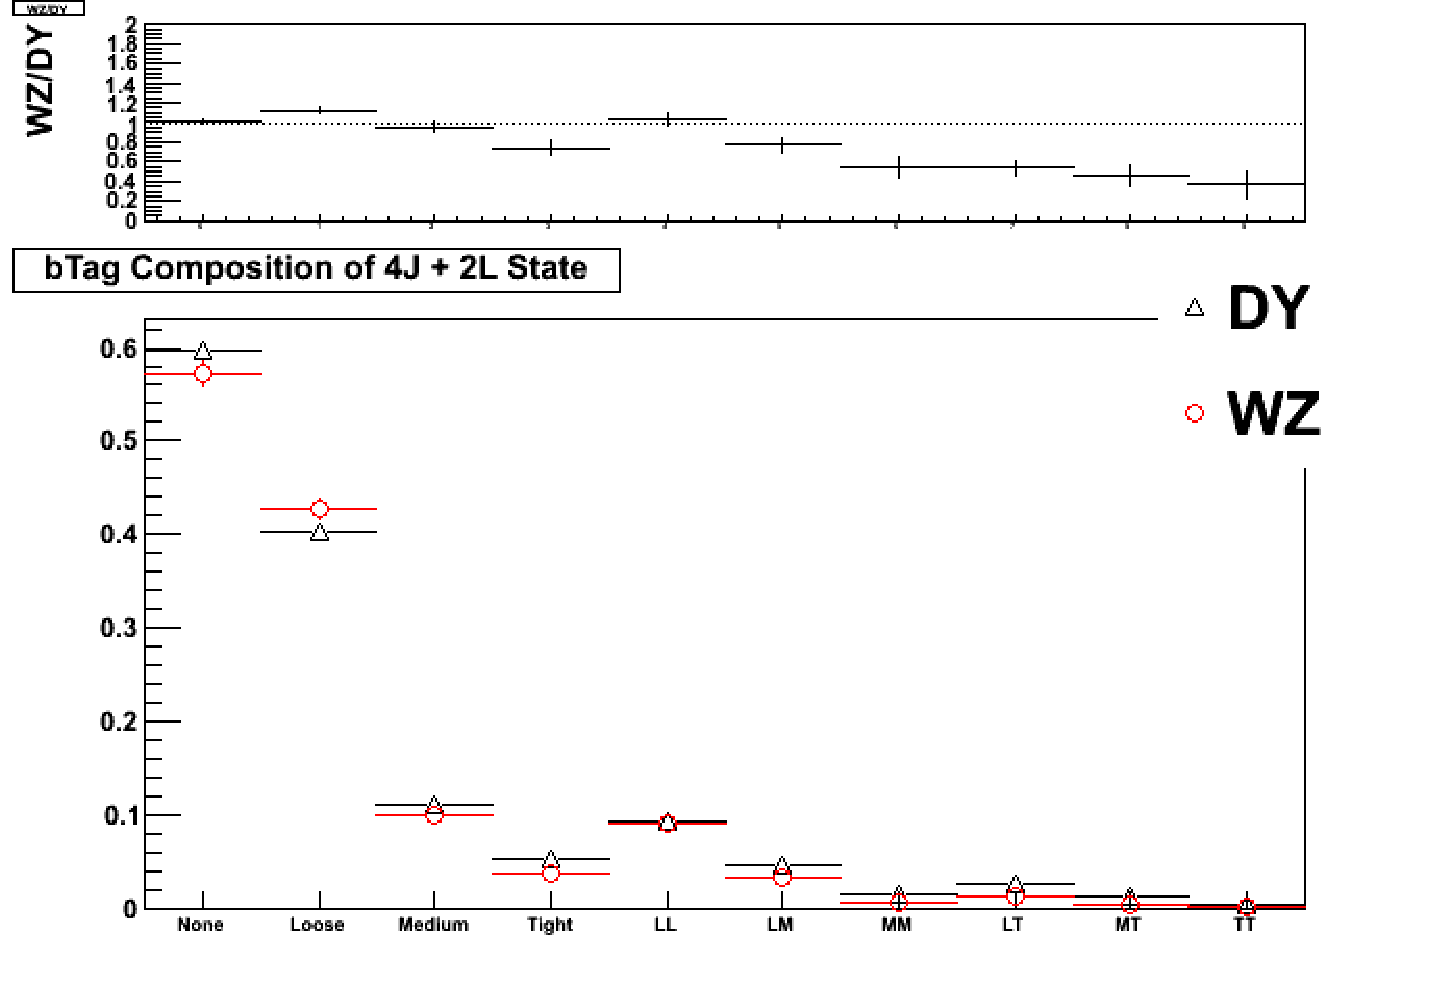
\includegraphics[width=0.90\linewidth]{Figs/WZ_Vs_DY_bComposition.pdf}
%\caption{\label{fig:wz_v_dy_btags}
%The b-tag composition of WZ and Z events in MC. In this plot, the first 2 bins (``None" and ``Loose") add up to the total number of events in the sample. The rest of the bins are a subset of the ``Loose" bin which shows the fraction of events with at least one CSV Loose b-tag. The bin labeled ``LL" means that this is the fraction of events with at least two CSV Loose b-tags. ``LM" means at least one Loose and one Medium, and so on. The WZ and Z samples are in good enough agreement for this purpose.
%}
%\end{center}
%\end{figure}

In data, control region events are required to pass the same mono- and di-lepton triggers as in the full analysis (there is a third lepton veto to make this region exclusive with the signal selection and thus the tri-lepton triggers are not used). The di-lepton event uses the same lepton requirements as are on the two leptons that are reconstructed as a Z in the tri-lepton selections in Section~\ref{sec:ElectronSelections}. Two mutually exclusive regions are defined, one with one CSV Loose b-tag and one CSV Medium b-tag used as the numerator of the ratio and one with a b-veto (i.e. zero Loose b-tags) used as the denominator of the ratio. These regions (particularly the b-tagged region) are contaminated with \ttbar \ events. A similar selection is made with the requirement that the di-lepton events contain two leptons that are different flavors (i.e. one electron and one muon), and this yield is subtracted from the Z like events to remove \ttbar \ contamination. The \ttbar \ estimate relies on the fact that the tops have final state decays into same flavor leptons at roughly the same rate as opposite flavor leptons. This creates a highly pure Z sample from which to determine the ratio. The constituents of the ratio are shown in both data and MC in Table ~\ref{tab:brate}

\begin{table}[ht!]
\caption{ \label{tab:brate} The constituent regions in the rate of b-tags in a 2L sample. An opposite flavor subtraction has been performed to create a more pure sample. Note the discrepancy between data and MC which will contribute to the systematic error on this method.}
\begin{center}
\begin{tabular}{c|cc}\hline
                                                         & 4J b-Veto                                & 4J (1Mb + 1Lb)\\
\hline \hline
W $\rightarrow \ell \nu$                       & 0.00$\pm$10.90      & 0.00$\pm$10.90    \\
VV $\rightarrow 2 \ell$                        & 951.43$\pm$4.30     & 216.37$\pm$2.15   \\
$t\overline{t}$                                & 2.40$\pm$2.37       & 5.48$\pm$7.80     \\
DY $\rightarrow 2 \ell$                        & 23678.13$\pm$224.34 & 2787.51$\pm$76.98 \\
%\hdashline
VZ $\rightarrow 3\ell$ or $4\ell$              & 28.38$\pm$0.50      & 3.65$\pm$0.17     \\
WWV                                            & 3.89$\pm$0.15       & 0.97$\pm$0.08     \\
%\hdashline
\ttX/tbZ/VZZ                                   & 5.21$\pm$0.26       & 10.00$\pm$0.80    \\
%\hdashline
\ttZ                                           & 3.48$\pm$0.26       & 33.97$\pm$0.83    \\
\hline \hline
Total from MC                                  & 24672.92$\pm$224.66 & 3057.94$\pm$78.18 \\
\hline
Data (19.5 fb$^{-1}$)                           & 24629.00$\pm$157.53 & 3874.00$\pm$75.54 \\
\hline
\end{tabular}
\end{center}
\end{table}
		
		
        		\subsubsection{Determining the Uncertainty in the Prediction from the b-tag Rate}
		A closure test on the accuracy of this method's predictions is performed in two ways. The first method is designed to show the integrity of the underlying assumption of the method that b-tag rates are independent of final states. The results are summarized in Table~\ref{tab:wz_z_brateclosure}. The rate of b-tags is measured in pure Z to two leptons with jets in MC and applied to a b-Veto region in our WZ, ZZ, and WWV samples with jets in MC. All three are included because they contribute and have enough statistics to be meaningful. This prediction is compared to the number of events measured in the two b-tag region for the pure WZ, ZZ, and WWV samples. The second test is designed to show the performance of the method in a sample with other types of processes than radiation producing jets that get b-tagged. The rate of b-tags is measured in a full cocktail of MC samples (with opposite flavor subtraction) with a two lepton and jets final state. This is then applied again to the WZ, ZZ, WWV samples with a three leptons and jets final state. The prediction is then compared to the measurement of three lepton and jets with b-tags in the same cocktail of MC. The results for the second test are summarized in Table~\ref{tab:mcsoup_brateclosure}.\\

\begin{table}[ht!]
\caption{ \label{tab:wz_z_brateclosure} Comparing the prediction of pure WZ, ZZ, and WWV MC events in a tri-lepton selection with b-tags from b-tag rates in pure Z MC sample.}
\begin{center}
\begin{tabular}{c|ccc}\hline
                                                                                               & Predicted            & Observed          & Pred. / Obs.\\
\hline \hline
WZ$\rightarrow 3\ell $ , ZZ$\rightarrow 4\ell$ , WWV  &  1.56$\pm$0.14 & 1.19$\pm$0.10 & 1.31$\pm$0.16\\		
\hline
\end{tabular}
\end{center}
\end{table}

\begin{table}[ht!]
\caption{ \label{tab:mcsoup_brateclosure} Comparing the prediction of pure WZ, ZZ, and WWV MC events in a tri-lepton selection with b-tags from b-tag rates in a cocktail of MC events in two lepton final state.}
\begin{center}
\begin{tabular}{c|ccc}\hline
                                                                                               & Predicted             & Observed          & Pred. / Obs.\\
\hline \hline
WZ$\rightarrow 3\ell $ , ZZ$\rightarrow 4\ell $ , WWV & $1.65 \pm 0.14$ & $1.19\pm0.10$ & $1.39 \pm 0.16$ \\
\hline
\end{tabular}
\end{center}
\end{table}

Based on the closure test results (Tables~\ref{tab:wz_z_brateclosure} and~\ref{tab:mcsoup_brateclosure}) and the agreement between data and MC shown in Table~\ref{tab:brate}, a 50\% systematic will be assessed on the prediction from this method.\\
		
		
        		\subsubsection{Predictions Due to the b-tag Rate Method}
		The columns from Table ~\ref{tab:brate} are used to predict the rate of b-tag events. The rate and the b-veto prediction region yields are listed in Table ~\ref{tab:brate_prediction} as well as the prediction.

\begin{table}[ht!]
\caption{ \label{tab:brate_prediction} Background predictions in data and MC for processes with b-tags that originate from radiation jets. Errors are statistical only.}
\begin{center}
\begin{tabular}{c|ccc}\hline
	   & Rate of b-tags	& Yields in b-Veto Sideband &	Bkg Prediction \\ \hline
Data   & 0.16$\pm$0.003	& 20.00$\pm$4.47            & 3.15+/-0.71 \\
MC	   & 0.12$\pm$0.003	& 14.38$\pm$2.45            & 1.78+/-0.31 \\
\hline
\end{tabular}
\end{center}
\end{table}

The prediction in Table~\ref{tab:brate_prediction} is further corrected by a scale factor determined by the Pred./Obs. in Table~\ref{tab:mcsoup_brateclosure}. The error remains the same, but the central value is now made better by correcting for the over prediction of the method. The final prediction is 2.27$\pm$0.51$_{st} \pm$1.14$_{sy}$.
		
